\section{Related Work}
\label{sec:related}

\begin{figure}[tbp]
	\hspace{0ex}
	\vspace{0ex}
	\centering
	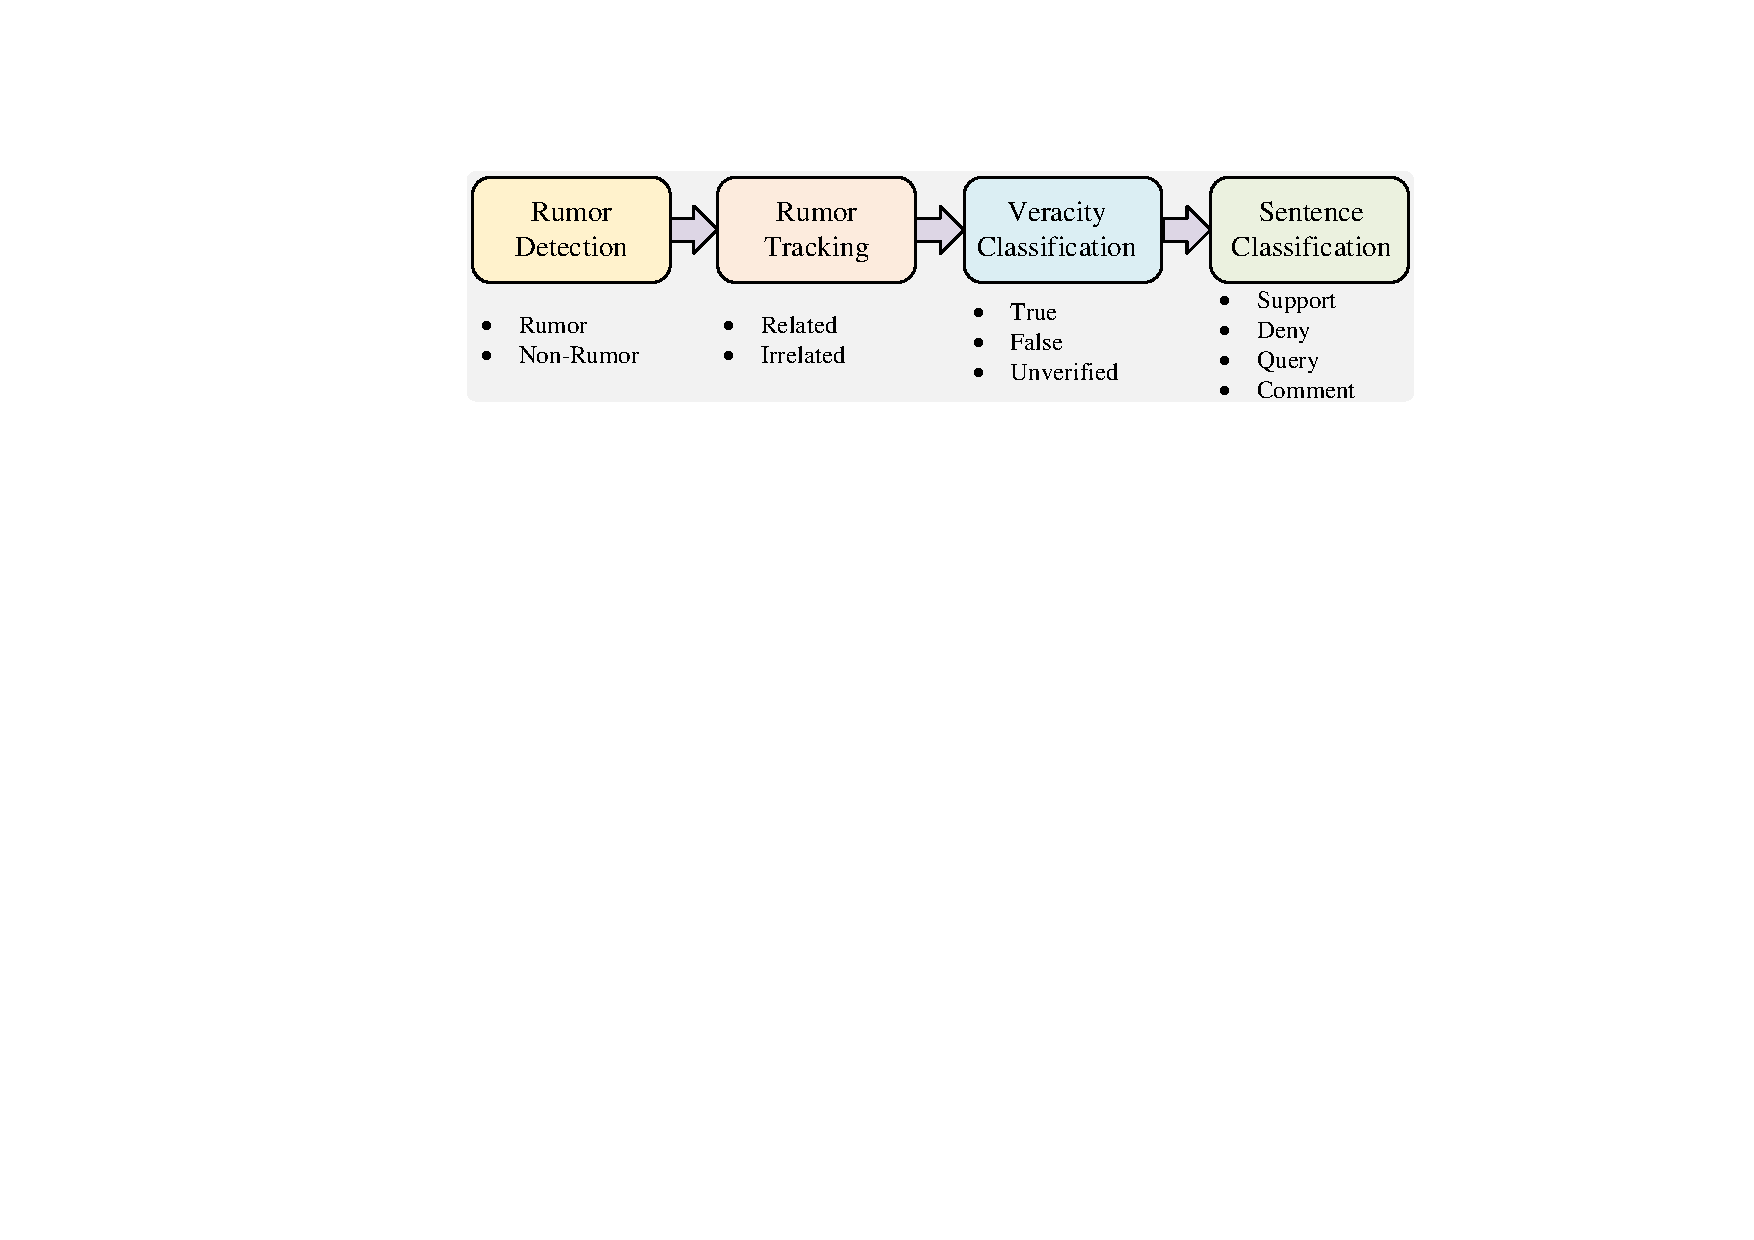
\includegraphics[width = \textwidth]{fig/pipeline}
	\caption{Pipeline of Rumor Detection Task}
	\label{fig:pipeline}
\end{figure}


\subsection{Rumor Tracking}
\label{sec:rumortracking}
The earliest Rumor tracking work is trace back to 2011. Several studies aims to find the relevant rumors for a known prior \cite{DBLP:journals/csur/ZubiagaABLP18}. Qazvinian et al. \cite{DBLP:conf/emnlp/QazvinianRRM11} explores three types of features including content-based, network-based, and microblog specific memes for identifying rumors. Hamidian et al. \cite{DBLP:journals/corr/abs-1912-08926} devise novel features and classify rumors with WEKA platform. These studies all focus on building features with simple classifiers. Cheng et al. \cite{DBLP:conf/www/ChengNB20} propose a multi-task learning model named VRoC and treat rumor tracking as one of the sub-tasks. VRoC is based on variational auto-encoder and uses tweet content as the input features. Overall, rumor tracking task is an important sub-task in rumor detection. However, compared to the other three sub-tasks, it attracts less attentions.

\subsection{Text Classification}
\label{sec:textclassification}
Text classification is a significant task in NLP area. In recent years, deep learning based text classification gets well developed. Kim et al. \cite{DBLP:conf/emnlp/Kim14} propose CNN based text classification. TextCNN use different sized kernels to capture different scaled gram features. Bojanowski et al. propose FastText  \cite{DBLP:journals/tacl/BojanowskiGJM17}, which can get embeddings of text in a short time. Inception \cite{DBLP:journals/corr/SzegedyLJSRAEVR14} uses larger width of network structure to capture more features. DPCNN \cite{DBLP:conf/acl/JohnsonZ17} adopts deeper network structure to get a better performance. From the recent studies, we can know that deep learning model achieves great success on text classification task.
